\item Tokyo-Fu was a large multi-divisional government institution overseeing the provision of public goods in Tokyo.
\begin{figure}
    \centering
    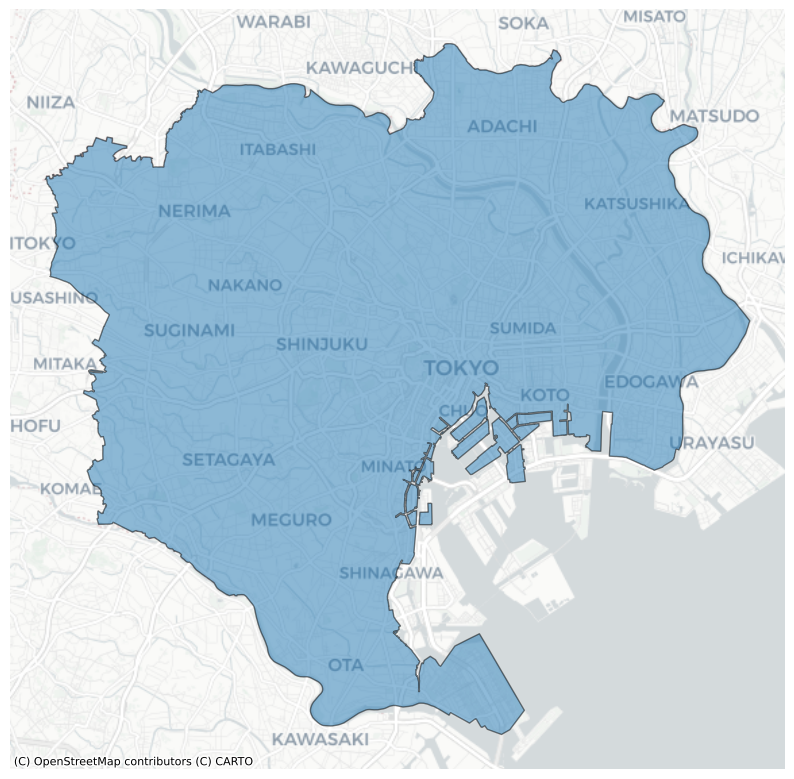
\includegraphics[width = \textwidth]{Background/MapOfTokyoFu.png}
    \caption{Map of Tokyo-Fu}
    \label{fig:enter-label}
\end{figure}

\item Hiring pool and promotion patterns differed for positions within the institution. The managerial positions often required qualification of the worker, which involved passing an internal examination. In contrast, non-managerial positions did not require qualifications and workers from local labor markets filled in the positions.

\item Promotion rules differed across workers' ranks. An internal committee consisting of employees decided the assignment of higher-ranked workers, whereas, for the lower-ranked workers, their managers decided their promotions at the end of their probation period. 

Certain positions required workers to hold a qualification in engineering. 

\item Expansion of military pressure led workers in Tokyo-Fu to leave their office roles to join the military. The army drafted soldiers based on age. All men were required to undergo a physical examination at 20 years old. The army assessed candidates based their physical health, and those with high scores were assigned to the military to serve for 2-3 years. Those with secondary scores were assigned to be the backup troops, who didn’t immediately serve but were called to supplement the army members who were injured or died. After finishing their military service, the ex-militants were still obliged to get drafted up until they turned 40 years old (The age limit was increased to 45 after 1943). 

\item Drafting was not predictable by the incumbent workers. I find no evidence of correlation between office attributes and drafting. 

